\documentclass[resume]{subfiles}


\begin{document}
\section{File system}
\subsection{Génération}
Squelette de rootfs dans \verb!workspace/nano/buildroot/system/skeleton!. Il est ensuite copié dans \verb!buildroot/output/target! et les fichiers nécessaires y sont ensuite ajoutés.\\
Une fois que tous les fichiers sont ajoutés, une image \verb!rootfs.xxx! est créé (xxx est ext4, squashfs, etc...)
=======

\subsection{}

\subsection{1. De connaître les différents types de systèmes de fichiers ainsi que leurs applications}

Pour les systèmes embarqués, il existe deux catégories de systèmes de fichiers :
\begin{enumerate}
    \item Volatiles en RAM
    \item Persitants sur des Flash (NOR et de plus en plus NAND)
\end{enumerate}

Deux technologies principales sont disponible sur les Flash :  
\begin{itemize}
    \item MTD (Memory Technology Device)
    \item MMC/SD-Card (Multi-Media-Card / Secure Digital Card)
\end{itemize}

\subsubsection{FS types}
\begin{figure}[H]
    \centering
    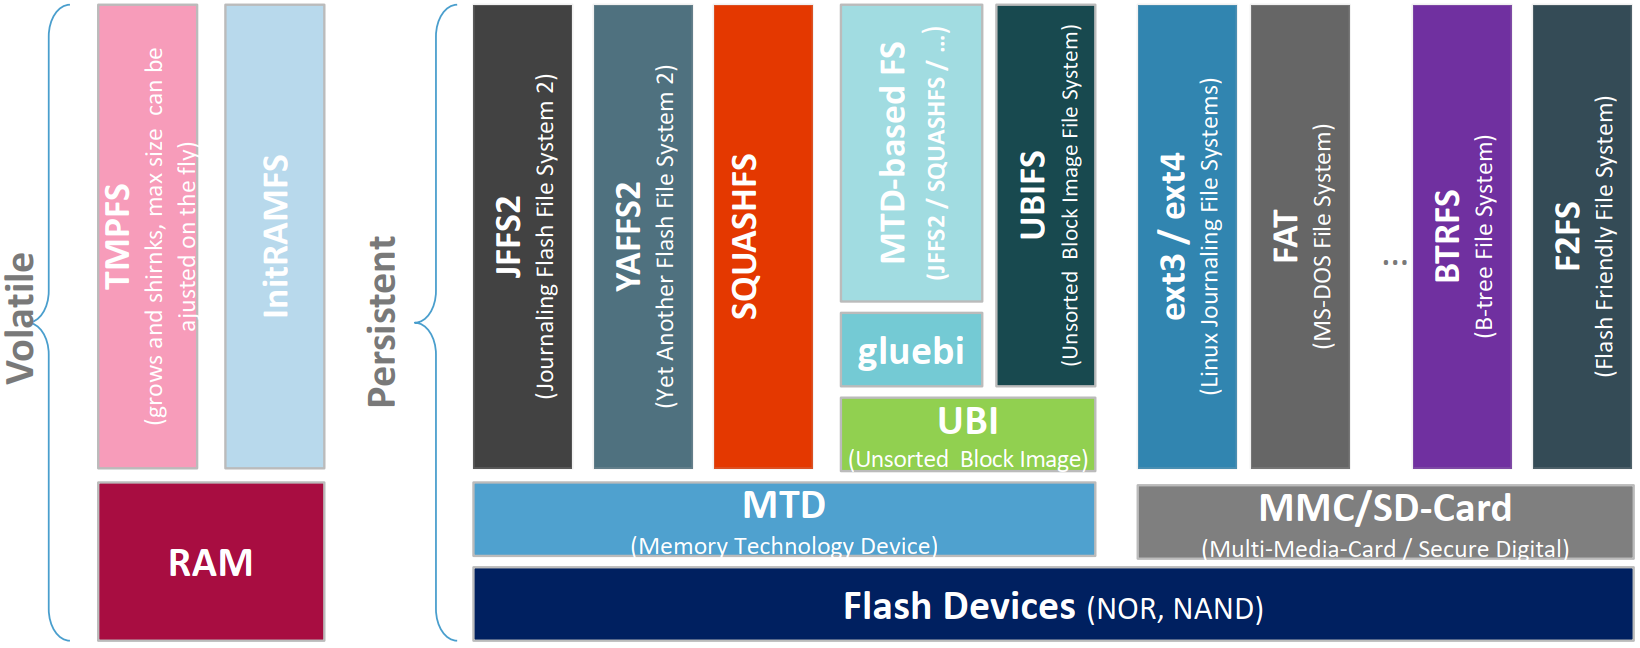
\includegraphics[width=0.7\columnwidth]{Figures/fileSystem/fileSystemType.PNG}
    \caption{FS type}
    \label{fig:fileSystemType}
\end{figure}

\subsubsection{Choix d'un FS}
\begin{figure}[H]
    \centering
    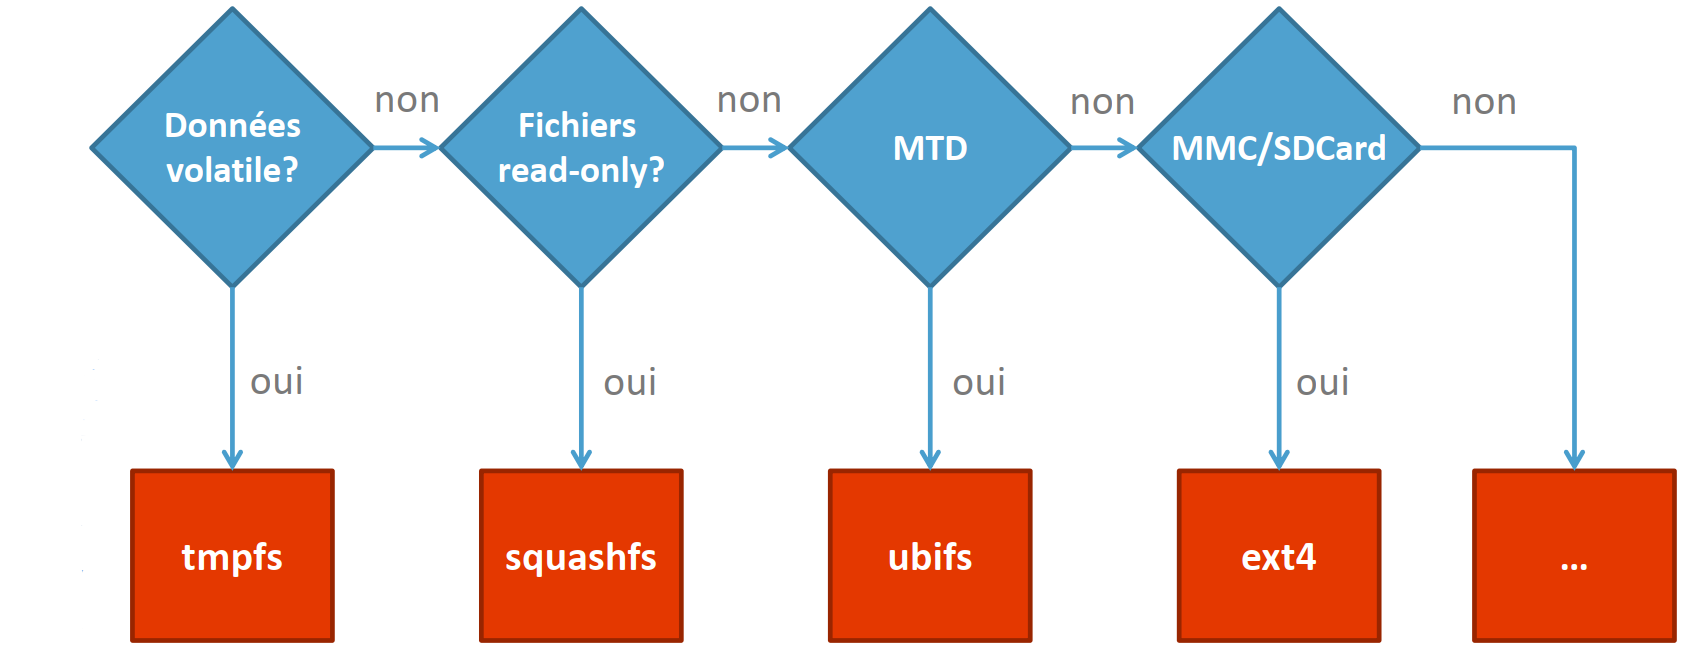
\includegraphics[width=0.7\columnwidth]{Figures/fileSystem/fileSystemChoice.PNG}
    \caption{FS type}
    \label{fig:fileSystemChoice}
\end{figure}

\subsubsection{MMC technologies}
MMC-eMMC-SD Card is composed by 3 elements
\begin{itemize}
    \item MMC interface: handle communication with host
    \item FTL (Flash translation layer)
    \item Storage area: array of NAND chips
\end{itemize}

\subsubsection{FTL}
FTL is a small controller running a firmware. Its main purpose is to transform logical sector addressing into NAND addressing. It also handles:
\begin{itemize}
    \item Bad block management
    \item Garbage collection.
    \item Wear levelling
\end{itemize}



\subsection{2. De connaître les caractéristiques des filesystems ext2-3-4, ainsi que les commandes associées}
“Filesystem considerations for embedded devices” is a good study about filesystems used on embedded systems.\\
This file system is very used in different Linux distribution.
\begin{itemize}
    \item EXT filesystem was created in April 1992 and is a file system for the Linux kernel
    \begin{itemize}
        \item Ext2 is not a journaled file system
        \item Ext2 uses block mapping in order to reduce file fragmentation (it allocates several free blocks)
        \item After an unexpected power failure or system crash (also called an unclean system shutdown), each mounted ext2 file system on the machine must be checked for consistency with the e2fsck program
    \end{itemize}
    \item EXT2 replaced it in 1993
    \begin{itemize}
        \item It was merged in the 2.4.15 kernel on November 2001
        \item Ext3 is compatible with ext2
        \item Ext3 is a journaled file system
        \item The ext3 file system prevents loss of data integrity even when an
        unclean system shutdown occurs
    \end{itemize}
    \item EXT4 arrived as a stable version in the Linux kernel in 2008
    \begin{itemize}
        \item ext4 is backward compatible with ext3 and ext2, making it possible to mount ext3 and ext2 as ext4
        \item Ext4 is included in the kernel 2.6.28
        \item Ext4 supports Large file system:
        \begin{itemize}
            \item Volume max: $2^60$ bytes
            \item File max: $2^40$ bytes
        \end{itemize}
        \item Ext4 uses extents (as opposed to the traditional block mapping scheme used by ext2 and ext3), which improves performance when using large files and reduces metadata overhead for large files
    \end{itemize}
\end{itemize}

\subsubsection{Ext4 commands}
\begin{lstlisting}[style=console,label={},caption={}]
    # Create a partition (rootfs), start 64MB, length 256MB
    sudo parted /dev/sdb mkpart primary ext4 131072s 655359s
    # Format the partition with the volume label = rootfs
    sudo mkfs.ext4 /dev/sdb1 -L rootfs
    # Modify (on the fly) the ext4 configuration
    sudo tune2fs <options> /dev/sdb1
    # check the ext4 configuration
    mount
    sudo tune2fs -l /dev/sdb1
    sudo dumpe2fs /dev/sdb1
    # mount an ext4 file system
    mount –t ext4 /dev/sdb1 /mnt/test // with default options
    mount –t ext4 –o defaults,noatime,discard,nodiratime,data=writeback,acl,user_xattr
    /dev/sdb1 /mnt/test
\end{lstlisting}

\subsubsection{Ext4 mount options and MMC/SD-Card}
\begin{itemize}
    \item filesystem options can be activated with the mount command (or to the /etc/fstab file)
    \item These options can be modified with tune2fs command
    \item Journaling: the journaling guarantees the data consistency, but it reduces the file system performances
    \item MMC/SD-Card constraints: In order to improve the longevity of MMC/SDCard, it is necessary to reduce the unnecessary writes
    \item Mount options to reduce the unnecessary writes (man mount) :
    \begin{itemize}
        \item noatime: Do not update inode access times on this filesystem (e.g., for faster access on the news spool to speed up news servers)
        \item nodiratime: Do not update directory inode access times on this filesystem
        \item relatime: this option can replace the noatime and nodiratime if an application needs the access time information (like mutt)
    \end{itemize}
\end{itemize}
Mount options for the journaling (man ext4):
\begin{itemize}
    \item Data=journal: All data is committed into the journal prior to being written into the main filesystem (It is the safest option in terms of data integrity and reliability, though maybe not so much for performance
    \item Data=ordered: This is the default mode. All data is forced directly out to the main file system before the metadata being committed to the journal
    \item Data=writeback: Data ordering is not preserved - data may be written into the main filesystem after its metadata has been committed to the journal. It guarantees internal filesystem integrity, however it can allow old data to appear in files after a crash and journal recovery.
    \item Discard: Use discard requests to inform the storage that a given range of blocks is no longer in use. A MMC/SD-Card can use this information to free up space internally, using the free blocks for wear-levelling.
    \item acl: Support POSIX Access Control Lists
    \item user_xattr: Support "user." extended attributes
    \item default: rw, suid, dev, exec, auto, nouser, and async
    \begin{itemize}
        \item rw : read-write
        \item suid : Allow set-user-identifier or set-group-identifier bits
        \item dev : Interpret character or block special devices on the filesystem
        \item exec : Permit execution of binaries
        \item auto : Can be mounted with the -a option (mount –a)
        \item nouser : Forbid an ordinary (i.e., non-root) user to mount the filesystem
        \item async : All I/O to the filesystem should be done asynchronously
    \end{itemize}
\end{itemize}

\subsubsection{/etc/fstab file}
File \textbf{/etc/fstab} contains descriptive information about the filesystems the system can mount
\begin{itemize}
    \item <file system> : block special device or remote filesystem to be mounted
    \item <mount pt> : mount point for the filesystem
    \item <type> : the filesystem type
    \item <options> : mount options associated with the filesystem
    \item <dump> : used by the dump (backup filesystem) command to determine whichfilesystems need to be dumped (0 -> no backup)
    \item <pass> : used by the fsck (8) program to determine the order in which filesystem checks are done at reboot time. The root filesystem should be specified with 1, and other filesystems should have a 2. if <pass> is not present or equal 0 -> fsck willassume that the filesystem is not checked.
    \item Field options: It contains at least the type of mount plus any additional options appropriate to the filesystem type.
\end{itemize}
Common for all types of file system are the options (man mount) :
\begin{itemize}
    \item auto : Can be mounted with the -a option (mount -a)
    \item defaults : Use default options: rw, suid, dev, exec, auto, nouser, and async
    \item nosuid : Do not allow set-user-identifier or set-group-identifier bits to take effect
    \item noexec : Do not allow direct execution of any binaries on the mounted file system
    \item nodev : Do not interpret character or block special devices on the file system
\end{itemize}


\subsection{3. D’expliquer les différents « files systems » utilisés dans les systèmes embarqués (ext2-3-4, BTRFS, F2FS, NILFS2, XFS, ZFS, …)}

\subsubsection{BTRFS (B-Tree filesystem)}
\begin{itemize}
    \item BTRFS is a “new” file system compared to EXT. It is originally created by Oracle in 2007, it is a B-Tree filesystem
    \item It is considered stable since 2014
    \item Since 2015 BTRFS is the default rootfs for openSUSE
    \item BTRFS inspires from both Reiserfs and ZFS
    \item Theodore Ts’o (ext3-ext4 main developer) said that BTRFS has a better direction than ext4 because "it offers improvements in scalability, reliability, and ease of management"
\end{itemize}

\subsubsection{F2FS (Flash-Friendly File System)}
It is a log filesystem. It can be tuned using many parameters to allow best handling on different supports.\\
F2FS features :
\begin{itemize}
    \item Atomic operations
    \item Defragmentation
    \item TRIM support (reporting free blocks for reuse)
\end{itemize}

\subsubsection{NILFS2 (New Implementation of a Log-structured File System)}
\begin{itemize}
    \item Developed by Nippon Telegraph and Telephone Corporation
    \item NILFS2 Merged in Linux kernel version 2.6.30
    \item NILFS2 is a log filesystem
    \item CoW for checkpoints and snapshots
    \item Userspace garbage collector
\end{itemize}

\subsubsection{XFS (Flash-Friendly File System)}
XFS was developed by SGI in 1993.
\begin{itemize}
    \item Added to Linux kernel in 2001
    \item On disk format updated in Linux version 3.10
    \item XFS is a journaling filesystem
    \item Supports huge filesystems
    \item Designed for scalability
    \item Does not seem to be handling power loss (standby state) well
\end{itemize}

\subsubsection{ZFS (Zettabyte ($10^21$)File System)}
ZFS is a combined file system and logical volume manager designed by Sun Microsystems.
\begin{itemize}
    \item ZFS is a B-Tree file system
    \item Provides strong data integrity
    \item Supports huge filesystems
    \item Not intended for embedded systems (requires RAM)
    \item License not compatible with Linux
\end{itemize}

\subsubsection{Conclusion}
Performances:
\begin{itemize}
    \item EXT4 is currently the best solution for embedded systems using MMC
    \item F2FS and NILFS2 show impressive write performances
\end{itemize}
Features:
\begin{itemize}
    \item BTRFS is a next generation filesystem
    \item NILFS2 provides simpler but similar features
\end{itemize}
Scalability:
\begin{itemize}
    \item EXT4 clearly doesn’t scale as well as BTRFS and F2FS
\end{itemize}

\begin{figure}[H]
    \centering
    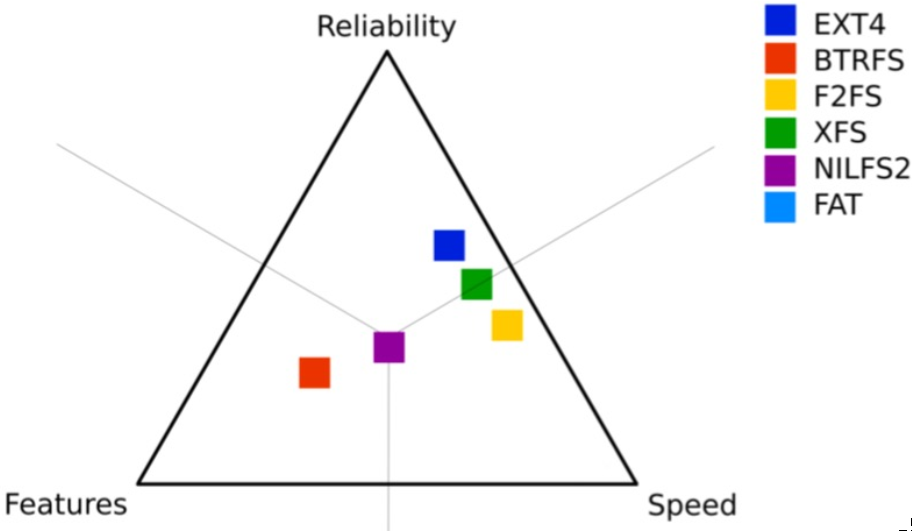
\includegraphics[width=0.7\columnwidth]{Figures/fileSystem/fsComp.PNG}
    \caption{FS Comparaison}
    \label{fig:fsComp}
\end{figure}

\subsection{4. Expliquer les « files system » de type Journal, B-Tree/CoW, log filesystem}

\subsubsection{Journalized filesystem}
A journalized filesystem keeps track of every modification in a journal in a dedicated area
\begin{itemize}
    \item EXT3, EXT4, XFS, Reiser4
    \item Journal allows to restore a corrupted filesystem
    \item Modifications are first recorded in the journal
    \item Modifications are applied on the disk
    \item If a corruption occurs: The File System will either keep or drop the
    modifications
    \begin{itemize}
        \item Journal is consistent : we replay the journal at mount time
        \item Journal is not consistent : we drop the modifications
    \end{itemize}
\end{itemize}
\subsubsection{B-Tree filesystem}
\begin{itemize}
    \item ZFS, BTRFS, NILFS2
    \item B+ tree is a data structure that generalized binary trees
    \item CoW (Copy on Write) is used to ensure no corruption occurs at runtime :
    \begin{itemize}
        \item The original storage is never modified. When a write request is made, data is written to a new storage area
        \item Original storage is preserved until modifications are committed
        \item If an interruption occurs during writing the new storage area, original storage can be used
    \end{itemize}
\end{itemize}

\begin{figure}[H]
    \centering
    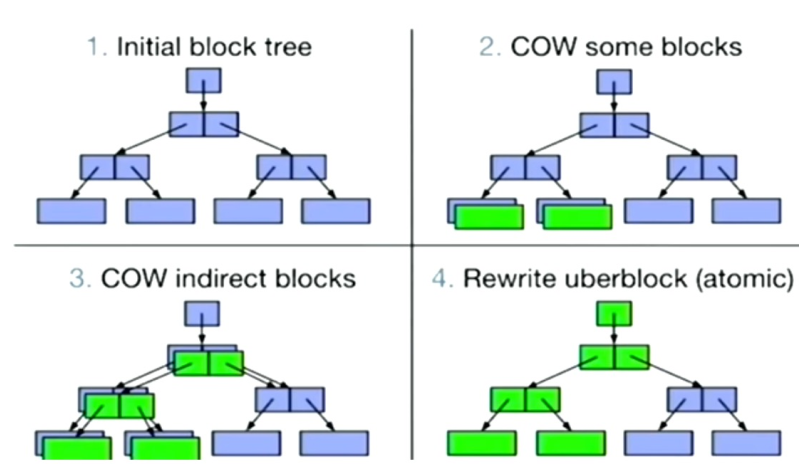
\includegraphics[width=0.7\columnwidth]{Figures/fileSystem/b-tree.png}
    \caption{B-tree type FS execution}
    \label{fig:b-tree}
\end{figure}

\subsubsection{Log filesystem}
Log-structured filesystems use the storage medium as circular buffer and new
blocks are always written to the end.
\begin{itemize}
    \item F2FS, NILFS2, JFFS2, UBIFS
    \item Log-structured filesystems are often used for flash media since they will naturally perform wear-levelling
    \item The log-structured approach is a specific form of copy-on-write behavior
\end{itemize}

\begin{figure}[H]
    \centering
    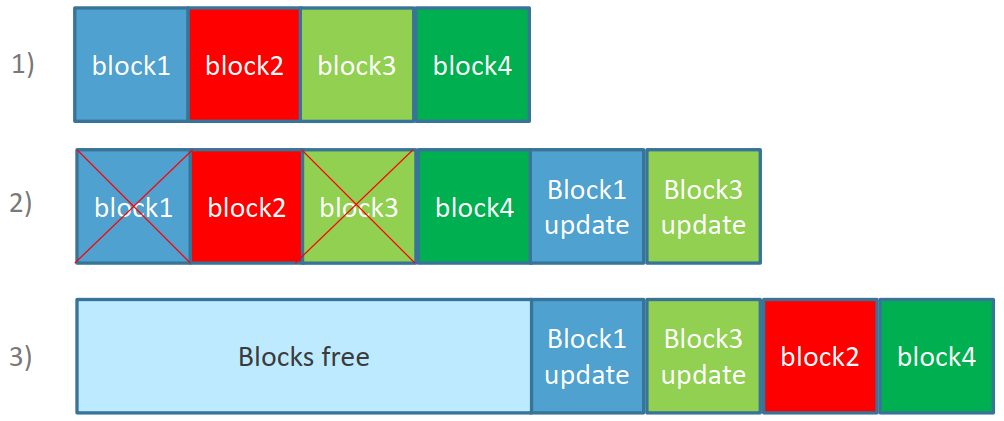
\includegraphics[width=0.7\columnwidth]{Figures/fileSystem/log_fs.png}
    \caption{log_fs type FS execution}
    \label{fig:log_fs}
\end{figure}
\begin{enumerate}
    \item Initial state
    \item Block 1-3 are updated, old blocks 1-3 are not used
    \item Garbage copies block2 and 4, and frees old block1-2-3-4
\end{enumerate}

\subsection{5. De connaître les caractéristiques du filesystem Squashfs, ainsi que les commandes associées}
\
begin{itemize}
    \item Squashfs is a compressed read-only filesystem for Linux
    \item Squashfs versions
    \begin{itemize}
        \item Squashfs 2.0 and squashfs 2.1: 2004, kernel 2.2
        \item Squashfs 3.0: 2006, kernel 2.6.12
        \item Squashfs 4.2: 2011, kernel 2.6.29
    \end{itemize}
    \item It uses gzip, lzma, lzo, lz4 and xz compression to compress files, inodes and directories
    \item SquashFS 4.0 supports 64 bit filesystems and files (larger than 4GB), full uid/gid information, hard links and timestamps
    \item Squashfs is intended for general read-only filesystem use, for archival use, and in embedded systems with small processors where low overhead is needed
    \item 
\end{itemize}

\begin{figure}[H]
    \centering
    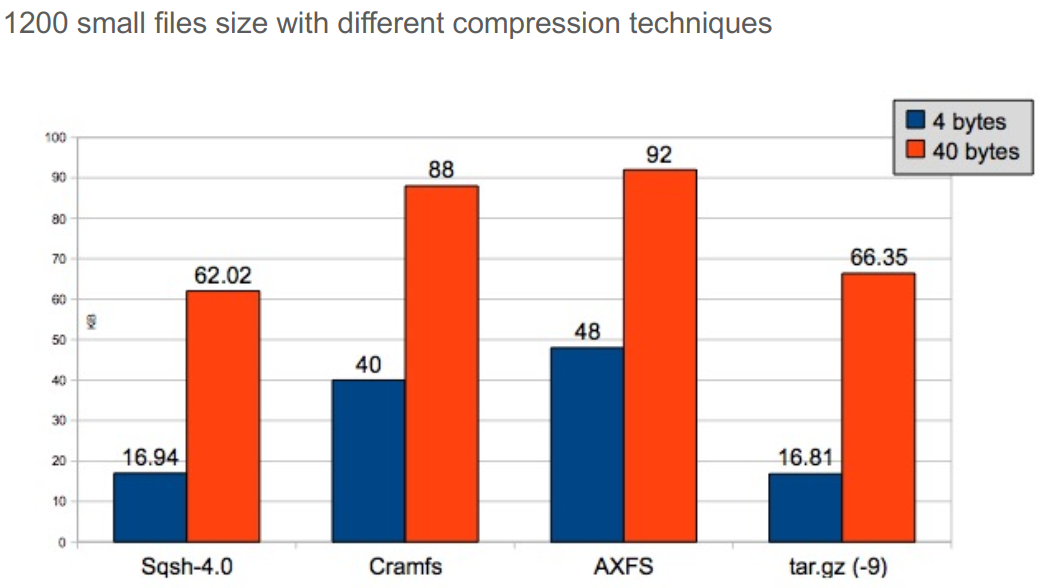
\includegraphics[width=0.7\columnwidth]{Figures/fileSystem/squashSystPerf.png}
    \label{fig:squashSystPerf}
\end{figure}

\subsubsection{Create and use squashed file systems}
\begin{enumerate}
    \item Create the squashed file system dir.sqsh for the regular directory /data/config/ :
    \begin{lstlisting}[style=console,label={},caption={}]
        bash# mksquashfs /data/config/ /data/dir.sqsh
    \end{lstlisting}
    \begin{figure}[H]
        \centering
        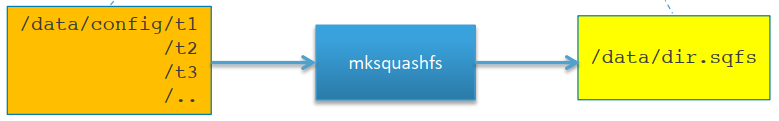
\includegraphics[width=0.7\columnwidth]{Figures/fileSystem/msquashfsCom.png}
        \label{fig:msquashfsCom}
    \end{figure}
    \item The mount command is used with a loopback device in order to read the squashed file system dir.sqsh
    \begin{lstlisting}[style=console,label={},caption={}]
        bash# mkdir /mnt/dir
        bash# mount –o loop –t squashfs /data/dir.sqsh /mnt/dir
        bash# ls /mnt/dir
    \end{lstlisting}
    \item It is possible to copy the dir.sqsh to an unmounted partition (e.g. /dev/sdb2) with the dd command and next to mount the partition as squashfs file system
    \begin{lstlisting}[style=console,label={},caption={}]
        bash# umount /dev/sdb2
        bash# dd if=dir.sqsh of=/dev/sdb2
        bash# mount /dev/sdb2 /mnt/dir -t squashfs
        bash# ls /mnt/dir
    \end{lstlisting}
\end{enumerate}

\subsection{6. De connaître les caractéristiques du filesystem tmpfs, ainsi que les commandes associées}
\begin{itemize}
    \item Tmpfs is a file system which keeps all files in virtual memory
    \item Everything in tmpfs is temporary in the sense that no files will be created on your hard drive. If you unmount a tmpfs instance, everything stored therein is lost.
    \item tmpfs puts everything into the kernel internal caches and grows and shrinks to accommodate the files it contains and is able to swap unneeded pages out to swap space. It has maximum size limits which can be adjusted on the fly via 'mount -o remount ...’
    \item If you compare it to ramfs you gain swapping and limit checking. Another similar thing is the RAM disk (/dev/ram*), which simulates a fixed size hard disk in physical RAM, where you have to create an ordinary filesystem on top. Ramdisks cannot swap and you do not have the possibility to resize them
\end{itemize}

\subsubsection{Devtmpfs}
\begin{itemize}
    \item devtmpfs is a file system with automatically populates nodes files (/dev/…) known by the kernel.
    \item This means, it is not necessary to have udev running nor to create a static /dev layout with additional, unneeded and not present device nodes.
    \item Instead the kernel populates the appropriate information based on the known devices.
    \item The kernel executes this command : mount -n -t devtmpfs devtmpfs /dev
    \item /dev is automatically populated by the kernel with its known devices
    \begin{lstlisting}[style=console,label={},caption={}]
        # ls /dev
        autofs ptypf tty47
        btrfs-control random tty48
        bus rtc0 tty49
        console shm tty5
        cpu_dma_latency snapshot tty50
    \end{lstlisting}
\end{itemize}

\subsection{7. De connaître les caractéristiques du filesystem LUKS, ainsi que les commandes associées}


\subsection{8. Savoir expliquer la gestion des clés de LUKS 42}


\subsection{9. De connaître les caractéristiques du filesystem InitramFS, ainsi que les commandes associées}


\subsection{10. De savoir créer un initramFS}


\end{document}